\chapter{Evaluation}
\label{ch:Evaluation}
\chaptertoc
\noindent

Chapter $6$ describes performance evaluation and experiments, comparing our load balancing methods based on the proactive approach with the existing balancing methods. The metrics for evaluation include imbalance ratio and speedup in completion time. We evaluate the speedup by the ratio between baseline (no balancing) and applied methods, such as work stealing, reactive task offloading, proactive task offloading. In detail, this chapter is outlined by
\begin{enumerate}
	\item Presenting the environmental setup in Section \ref{sec:environmental_experiments}.
	\item Presenting the evaluation of online load prediction that provides knowledge for proactive task offloading methods, in Section \ref{sec:online_prediction_evaluation}.
	\item Presenting the comparison results between our methods and the existing methods in Section \ref{sec:evaluate_proact_lb}.
	\item Presenting the evaluation of co-scheduling tasks across multiple applications in Section \ref{sec:evalulate_coschedule_tasks}, which is considered as an extension based on our proactive load balancing approach.
\end{enumerate}

These experiments are performed in three different HPC clusters using synthetic micro-benchmarks and a realistic HPC application. 

\section{Environmental Experiments} \label{sec:environmental_experiments}

We configure and perform experiments on three different HPC systems at the Leibniz Supercomputing Centre (LRZ), namely CoolMUC2, SuperMUC-NG and BEAST. The overview of these systems is already mentioned in Chapter \ref{ch:perfmodel} on Page \pageref{footnote:lrz_coolmuc}. However, to give a detailed specification of hardware and software stack, we present Table \ref{tab:exp_system_env}, describing more information such as processor type, the number of CPU sockets (\# sockets), number of cores per socket (\# core per socket), memory volume, and the maximum bandwidth (Max. bandwidth - $B$) measured by using the OSU benchmark \cite{panda2021mvapich}.\\

\begin{table}[t]
\centering
\caption{The specification of systems for runing experiments.}
\scalebox{0.95}{
\begin{tabular}{|m{4.1cm}|m{2.8cm}|m{3.0cm}|m{4.0cm}|}
\hline
\textbf{Specification} & \textbf{CoolMUC2} & \textbf{SuperMUC-NG} & \textbf{BEAST}       \\ \hline
Processor              & Intel Xeon E5-2697 v3 \@ 2.60GHz & Intel Skylake Xeon Platinum 8174 \@ 2.40GHz & featured with different processors, e.g., AMD Rome EPYC 7742, ARM ThunderX2, Fujitsu A64FX, Intel CooperLake \\ \hline
\# sockets             & 2  &  2  & 2(AMD), 2(ARM), 1(A64FX), 4(Intel)     \\ \hline
\# cores per socket    & 14 &  28 & 64(AMD), 32(ARM), 48(A64FX), 24(Intel) \\ \hline
Memory  & 64 &  96 (thin nodes), 768 (fat nodes) & 512(AMD), 512(ARM), 32(A64FX), 768(Intel)    \\ \hline
Network Infrastructure & FDR14 Infiniband & OmniPath 100Gb/s & HDR InfiniBand 200Gb/s                          \\ \hline
Max. bandwidth (B) (measured with OSU Benchmark \cite{panda2021mvapich}) & 6.52 GB/s & 12.07 GB/s & 22.03 GB/s \\ \hline
Operating System (OS) & SLES15 SP1 Linux & Suse Linux (SLES) & Suse SLES (AMD, Intel nodes), CentOS 8 (ARM, A64FX nodes)     \\ \hline
\end{tabular}}
\label{tab:exp_system_env}
\end{table}

The main difference between these systems is the interconnection, distinct by different technologies. CoolMUC2 uses FDR14 Infiniband, an older technology with a bandwidth of $\approx$ $6.52$ GB/s. SuperMUC-NG is higher with $12.07$ GB/s, and BEAST is a better system featured with a new Infiniband technology $\approx$ $22.03$ GB/s. Especially in the BEAST system, it has different types of computing architectures, featuring two nodes of AMD processors (Rome EPYC 7742), two nodes of ARM ThunderX2, eight nodes or a so-called small cluster with Fujitsu A64FX, and two nodes of Intel CooperLake CPU. However, we do not use all of the nodes on BEAST, only selecting several nodes with the same architectures to run the experiments.

% -----------------------------------------------------
\newpage
% -----------------------------------------------------

Regarding micro-benchmarks, we use the following kernels to define tasks.
\begin{itemize}
	\item \texttt{MxM}: matrix multiplication, which is mentioned as an example for our illustration in the previous chapters. A task is defined by a matrix multiplication compute kernel.
	\item \texttt{Nbody}: N-body simulation, which is a simulation of a dynamical system of particles. Tasks in \texttt{Nbody} are defined by different compute kernels, such as Nbody solver and force calculation.
	\item \texttt{Jacobi:} Jacobi solver, which refers to the Jacobi method in numerical linear algebra. The compute kernels in the Jacobi solver define tasks.
\end{itemize}

Regarding the realistic use case, we use Sam(oa)$^2$ \cite{Meister2016AMRSamoa} as introduced in Chapter \ref{ch:PADLB}, Page \pageref{subsubsec:samoa-online-prediction}. Sam(oa)$^2$ is a simulation framework developed through the concept of Space-filling curves and Adaptive Mesh Refinement for Oceanic Applications in HPC. This framework features hybrid MPI+OpenMP parallelization based on the Sierpinski order. The Sam(oa)$^2$ authors focus on providing a dynamically adaptive solver for 2D Partial Differential Equations (PDEs).\\

In terms of scientific simulation, there are two popular scenarios using Sam(oa)$^2$: 
\begin{itemize}
	\item simulating multiphase flow in porous media.
	\item simulating environmental issues, such as tsunami wave propagation and earthquake, based on solving shallow water equations.
\end{itemize}

In our experiments, we deploy Sam(oa)$^2$ as a real use case, simulating related oceanic problems such as tsunami wave propagation, oscillating lake. The design of Sam(oa)$^2$ aims at memory efficiency, where the complexity of the stack\&stream approach is hidden while providing flexibility for multiple discretization methods. There are different variants of Sam(oa)$^2$ researched for a certain optimization purpose. In this thesis, we refer to using a new optimized version called ADER-DG \cite{rannabauer2018samoaaderdg} because it is said to be optimized with the application of the ADER Discontinuous Galerkin method for simulating tsunamis. Similar to Sam(oa)$^2$, there are several libraries and frameworks, e.g., Peano \cite{bungartz2010peano}, PDELab in DUNE \cite{blatt2007dune}.\\

Related to task definition and execution, the Sam(oa)$^2$ framework employs the workflow of traversing grid. The grid is sub-partitioned into sections. All sections are distributed in distributed memory systems over multiple processes. With task-based parallel programming models, threads in a process are execution units that traverse these sections. Traversing a section is considered as a computational task. These computations are characterized as independent tasks in Chameleon. Before execution, the canonical approach in Sam(oa)$^2$ itself divides the whole grid into equal parts over processes. Following that, tasks within a process are uniform or equal load, but the tasks from different processes might not have the same load values. Furthermore, Sam(oa)$^2$ already has several balancing techniques built in the framework relying on its cost models. However, our context is assumed to encounter performance slowdown; therefore, this leads to a new imbalance at runtime.

\section{Online Load Prediction Evaluation} \label{sec:online_prediction_evaluation}

This section shows an evaluation of our online load prediction scheme described in Subsection \ref{subsec:ml-based-design}. The experiments consist of \texttt{MxM} matrix multiplication and Sam(oa)$^2$. For the evaluation, we specify two criteria:
\begin{itemize}
	\item Accuracy: the accuracy of prediction models. The metric accounting for accuracy is loss, which alludes to the difference between real and predicted values.
	\item Overhead: the overhead of training and inferencing prediction models. The unit accounting for overhead is time in microseconds, milliseconds, or seconds, depending on the length of completion time.
\end{itemize}

There are different metrics to calculate the loss in machine learning \cite{naser2021errormetricsml}. We use the following loss metrics:
\begin{itemize}
	\item MAE: Mean Absolute Error. MAE calculates the absolute difference between actual and predicted values.
	\item MSE: Mean Squared Error. MSE calculates the squared difference between actual and predicted values.
	\item RMSE: Root Mean Squared Error. RMSE is a simple square root of MSE.
	\item R2score: R Squared. R2score is a metric that explains the performance of prediction models, calculating how much a regression line is better than a mean line in prediction.
\end{itemize}

For the overhead of training and inferencing, we compare the application completion time with the training and inferencing times. This overhead is important because if its value is too high, not only the load balancing module is affected but also the execution of our application.\\

Our evaluation is divided into two groups of experiments, detailed in the following subsections.
\begin{enumerate} \label{enum:exp_vayring}
	\item Varying the scale parameters: the number of compute nodes and the number of threads per process. This group of experiments aims at the feasibility of applying machine learning in online load prediction by evaluating the accuracy. Simultaneously, we show that the accuracy and cost of training and loading the prediction model, are not greatly affected when increasing the computational scale.
	\item Varying the machine learning algorithms: Linear Regression, Ridge, Bayesian, and LARS (Least Angle Regression (Stage-wise/laSso)). These algorithms are classified as regression algorithms in machine learning \cite{bonaccorso2017mlalgorithms}. This group of experiments focuses not on accuracy but on flexibility in user-defined prediction models. We show that load prediction models can change based on users and specific applications. Thereby, in this group, we highlight that flexibility in applying different machine learning algorithms is feasible. Simultaneously, accuracy can be guaranteed when we understand our applications as well as prediction models.
\end{enumerate}

%\noindent \textbf{A. Varying scales of nodes and threads per process}\\
\subsection{Varying the scale parameters: the number of compute nodes and the number of threads per process}
\label{subsec:exp_loadpred_variedscales}

We perform three experiments that revolve around adjusting the number of compute nodes and the number of threads per process. These experiments include:
\begin{itemize}
	\item Experiment 1: is performed with \texttt{MxM} matrix multiplication, where we vary the number of compute nodes from 2 to 64. This experiment is performed on CoolMUC2, and the results are shown in Table \ref{tab:exp_online_pred_overhead_node_scale}. It is configured by the same number of tasks assigned to each process. To increase objectivity, we randomize the argument size of tasks, resulting in randomized wallclock execution time.  
	\item Experiment 2: is also performed with \texttt{MxM}, but we vary the number of threads per process. This experiment is performed with two nodes on the BEAST system because BEAST has AMD nodes featuring a multicore architecture with 64 physical cores per processor. This allows deploying multiple threads in a process. The experiment results are shown in Table \ref{tab:exp_online_pred_overhead_thread_scale}.
	\item Experiment 3: is performed with the realistic application, Sam(oa)$^2$, where we run Sam(oa)$^2$ to simulate oscillating lake over $100$ time steps (iterations). This experiment is used to evaluate the accuracy of online load prediction in a real use case. We again vary the number of compute nodes, and the results are shown in Figure \ref{fig:online_pred_results_samoa}.
\end{itemize}

In addition, the experiments with \texttt{MxM} can be reproduced with different imbalance scenarios through the number of assigned tasks per process and task data size. However, to evaluate load prediction, we only focus on the load of tasks and configure the same number of tasks per process, where task argument size is randomized to create randomized load values.\\

\begin{table}[t]
\centering
\caption{Evaluation of online load prediction for \texttt{MxM} matrix multiplication over the scale of compute nodes.}
\scalebox{0.95}{
\begin{tabular}{|m{1.8cm}|m{2.8cm}|m{2.6cm}|m{2.6cm}|}
\hline
\textbf{Node scales} & \textbf{avg(MSE loss)} & \textbf{training time (ms)} & \textbf{inference time (ms)} \\ \hline
2										 &  0.00059  &  458.209  &  0.1357    \\ \hline
4										 &  0.00038  &  478.609  &  0.1406    \\ \hline
8										 &  0.02888  &  502.514  &  0.1432    \\ \hline
16									 &  0.00470  &  320.179  &  0.1518    \\ \hline
32									 &  0.00618  &  277.506  &  0.1492    \\ \hline
64									 &  0.02130  &  346.579  &  0.1613    \\ \hline
\end{tabular}}
\label{tab:exp_online_pred_overhead_node_scale}
\end{table}

Table \ref{tab:exp_online_pred_overhead_node_scale} shows the prediction results of Experiment 1. It has four columns, where the compute node scale is shown in the column ``Node scales'', varied from $2$ to $64$ nodes. Accordingly, the next columns ``avg(MSE loss)'', ``training time'', and ``inference time'' show the results of loss values calculated by MSE, overhead by training time, and inferencing time in milliseconds.\\

On CoolMUC2, each node is deployed $2$ MPI processes. Each process spawns $13$ OpenMP threads to execute tasks and $1$ thread (pthread) to dedicate communication ($Tcomm$). Given a distribution of tasks, we assign $200$ tasks on each process. For the prediction model in this case, we use the task's argument sizes and CPU core frequencies for the input layer. Task wallclock execution time is configured for the output label. Note that the core frequencies of compute nodes on CoolMUC2 are safely configured ``fixedly''; therefore, they do not influence the prediction model. In this case, only matrix sizes affect the model's accuracy. Regarding the machine learning algorithm, $Tcomm$ is configured to use linear regression to train the prediction model. The results of Experiment 1 in Table \ref{tab:exp_online_pred_overhead_node_scale} show that:
\begin{itemize}
	\item The loss values over different node scales remain low and stable (around $\approx 0.02$). This highlights the feasibility of predicting load during execution, especially supporting load balancing.
	\item The training and inferencing time are also low and stable. The maximum training overhead is $\approx 500$ms, and the inferencing overhead is under $1$ms.
\end{itemize}
  
In our approach, the operations of $Tcomm$ are separate from the others; therefore, the overhead of deploying machine learning keeps little change over different experiments. Particularly, over node scales, we can see that training and inferencing time remain approximately. In fact, the cost of training might be a trouble if the dataset is large and complex. However, regarding online load prediction, we need to select influence factors that can be satisfied to help training. Therefore, we show that the number of parameters suitable for predicting load is not many, and a lightweight machine learning model to predict the load at runtime is possible.\\

\begin{table}[t]
\centering
\caption{Evaluation of online load prediction for \texttt{MxM} over the scale of threads per process.}
\scalebox{0.95}{
\begin{tabular}{|m{2.2cm}|m{2.2cm}|m{2.8cm}|m{2.7cm}|m{2.7cm}|}
\hline
\textbf{\#threads per process} & \textbf{real $R_{imb}$} & \textbf{predicted $R_{imb}$} & \textbf{training time (ms)} & \textbf{inference time (ms)} \\ \hline
2										 &  0.0311  &  0.0108  &  18.156   &  0.0257    \\ \hline
4										 &  0.2706  &  0.3863  &  18.218   &  0.0103    \\ \hline
8										 &  0.5384  &  0.5079  &  19.804   &  0.0215    \\ \hline
16									 &  0.3502  &  0.2298  &  19.793   &  0.0199    \\ \hline
32									 &  0.5815  &  0.5442  &  19.807   &  0.0192    \\ \hline
64									 &  0.4245  &  0.3111  &  20.951   &  0.0229    \\ \hline
\end{tabular}}
\label{tab:exp_online_pred_overhead_thread_scale}
\end{table}

Table \ref{tab:exp_online_pred_overhead_thread_scale} shows the results of Experiment 2, varying the number of task-execution threads per process. It has five columns, where the first column indicates the number of threads, ``\#threads per process''. The next columns show ``real $R_{imb}$'', ``predicted $R_{imb}$'', ``training time'', and ``inference time'' respectively. The real $R_{imb}$ values are calculated by the real (observed) total load values of processes, while the predicted $R_{imb}$ values are calculated by the predicted total load values of processes. Notably, this experiment presents the load prediction of each task ($w$) in \texttt{MxM}; therefore, the predicted total load values per process can be calculated by summing up all values $w$ that belong to a process. The results of Experiment 2 in Table \ref{tab:exp_online_pred_overhead_thread_scale} highlight that:

\begin{itemize}
	\item The difference between real and predicted $R_{imb}$ is low and optimistic, except for the case with the smallest scale, $2$ threads per process. This is because the real imbalance ratio is already too small. Other cases show again the feasibility of online load prediction over changing the number of threads executing tasks.
	\item The training and inferencing time on BEAST are smaller and more stable than in Experiment 1 (on CoolMUC2). This is partly from executing on BEAST; the core frequencies are not fixed, and the prediction model has an input parameter of core frequencies, which increases the accuracy of the machine learning model.
\end{itemize}

Overall, $Tcomm$ is asynchronously run with the other execution threads. Its overhead does not impact system-level configuration, e.g., node or thread scales. In terms of prediction accuracy, we show that considering influence features for online load prediction should be revised by users. Depending on a definition of tasks, users can define influence features better.\\

\begin{figure}[t]
\centering
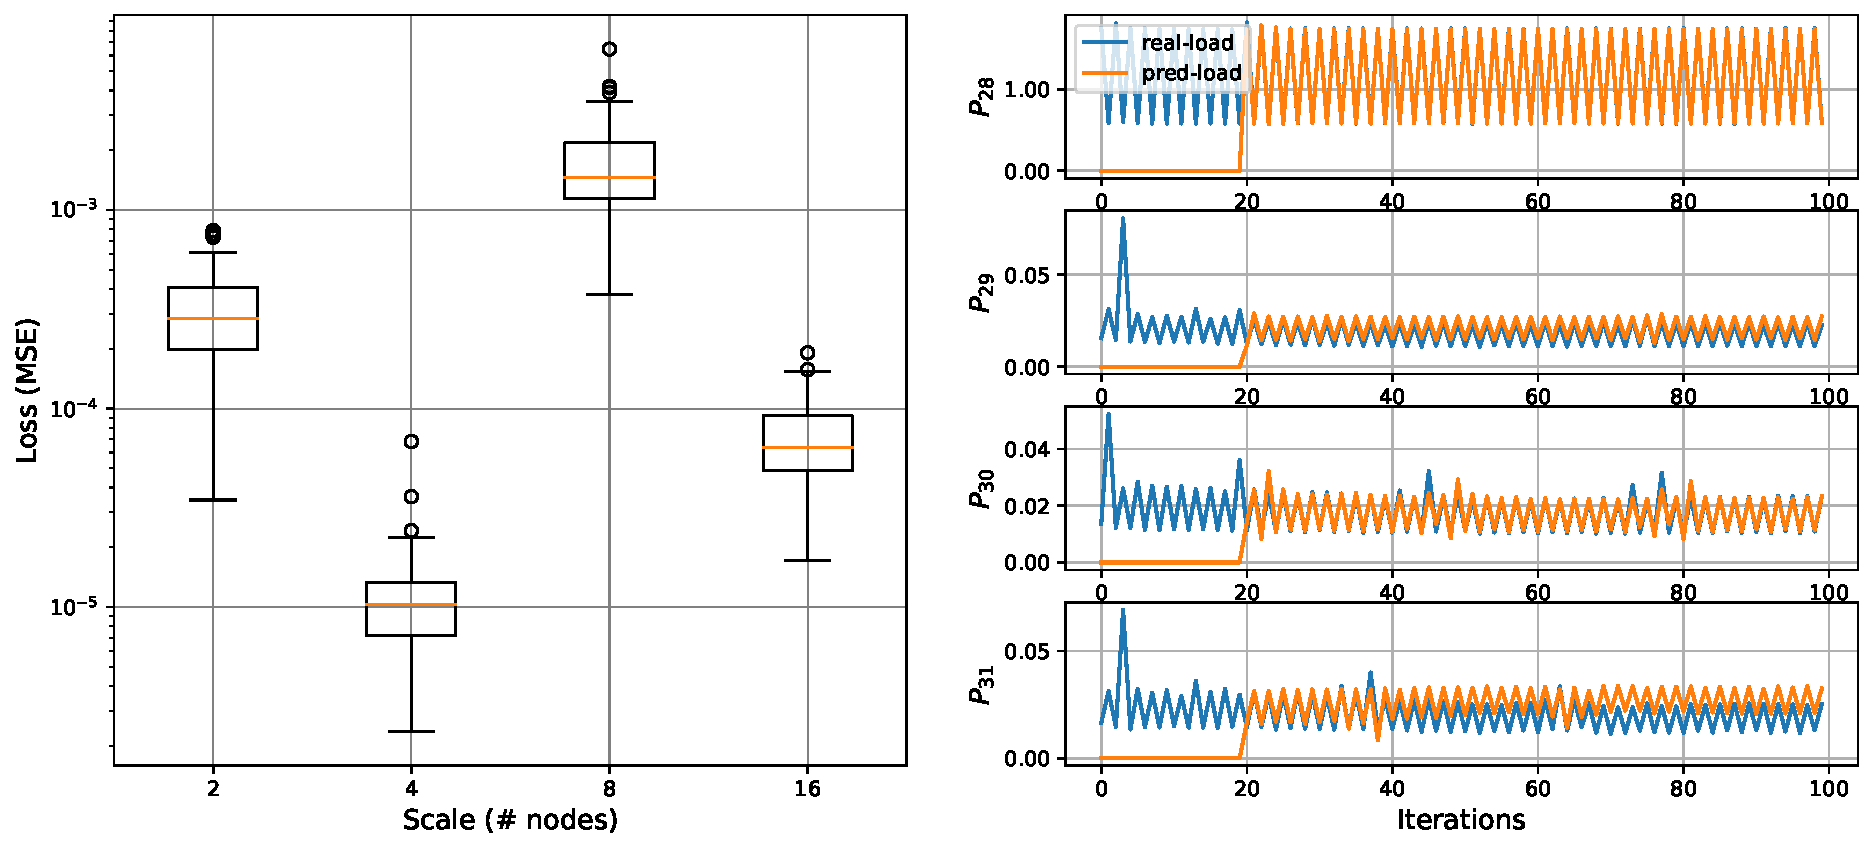
\includegraphics[scale=0.475]{./pictures/evaluation/eval_loss_and_realvspred_comparison_R28_R31.pdf}
\caption{Evaluation of online load prediction on Sam(oa)$^2$ when simulating oscillating lake.}
%\vspace{-1.0em}
\label{fig:online_pred_results_samoa}
\end{figure}

Figure \ref{fig:online_pred_results_samoa} shows the results of Experiment 3, running Sam(oa)$^2$ over $100$ time steps (iterations or iter for short). This experiment is performed on CoolMUC2, where the number of compute nodes is varied from $2$ to $16$. Unlike \texttt{MxM}, the predicted load of each process is based on the load value in previous iterations. We use $20$ first iterations for generating the dataset, then $Tcomm$ on each process trains the model afterward. The trained model is loaded at the $21^{st}$ iteration. Figure \ref{fig:online_pred_results_samoa} has two plots, where the left one shows a box plot of MSE loss values over different scales of compute nodes, and the right one illustrates the comparison between real and predicted load values in the case of $16$ nodes. In Figure \ref{fig:online_pred_results_samoa} (left), the x-axis indicates the labels of node scale, while the y-axis indicates MSE values. In Figure \ref{fig:online_pred_results_samoa} (right), the x-axis indicates the iteration indices from $0$ to $99$, and the y-axis indicates the process labels along with the load values in seconds. The results in this experiment highlight that:
\begin{itemize}
	\item MSE loss again shows the feasibility when we predict the load values at runtime by a different prediction model. Particularly, it relies on the load in the previous iterations. The smaller loss determines a better prediction.
	\item The comparison between real and predicted load values emphasizes the applicability of machine learning when training prediction models at runtime. The iterations indexed from $0$ to $19$ are used to generate the dataset, in which we see the predicted values are zero. The results in Figure \ref{fig:online_pred_results_samoa} (right) correspond to the $16$-nodes scale, where each node is deployed $2$ processes, and we have $32$ processes in total. This figure only shows the results of $4$ in $32$ processes, i.e., $P_{28}$,  $P_{29}$,  $P_{30}$,  $P_{31}$, because the results of other processes are similar. Thus, it is not necessary to illustrate them all. Besides that, the presented results of $4$ processes also fit better with Figure \ref{fig:online_pred_results_samoa} on the left. Starting from iteration $20$, the total load values of processes are predicted. The blue line denotes observed values (real values), while the orange line shows predicted values.
\end{itemize}

These results show a positive outcome in general. Besides that, we conclude that the major point of load balancing is the load difference between the involved processes. Therefore, a very high-accuracy prediction is not a challenge; instead, we can rely on the load difference among processes to guide load balancing. Unlike several problems in computer vision or natural language processing, the high-accuracy prediction models are expected. In our context, the experiments above show that using load prediction results at runtime to balance the load is feasible.

% \noindent \textbf{Feasible to change machine learning algorithms and augment dataset to re-train the models} \\

%\noindent \textbf{B. Changing machine learning algorithms}\\
\subsection{Varying the machine learning algorithms}
\label{subsec:exp_change_mlalgs}

\begin{table}[t]
\caption{The evaluation of load prediction using different machine learning regression algorithms.}
\centering
\scalebox{0.9}{
\begin{tabular}{|l|llll|}
\hline
                    & \multicolumn{4}{l|}{\textbf{\texttt{MxM} Matrix Multiplication}}                                            \\ \hline
\textbf{Loss}       & \multicolumn{1}{l|}{\textbf{MAE}} & \multicolumn{1}{l|}{\textbf{MSE}} & \multicolumn{1}{l|}{\textbf{RMSE}} & \textbf{R2score} \\ \hline
Linear Regression   & \multicolumn{1}{l|}{0.23947} & \multicolumn{1}{l|}{0.12241} & \multicolumn{1}{l|}{0.34001} & 0.68828 \\ \hline
Ridge Regression    & \multicolumn{1}{l|}{0.23916} & \multicolumn{1}{l|}{0.12242} & \multicolumn{1}{l|}{0.33997} & 0.68828 \\ \hline
Bayesian Regression & \multicolumn{1}{l|}{0.26755} & \multicolumn{1}{l|}{0.14175} & \multicolumn{1}{l|}{0.36823} & 0.68828 \\ \hline
LARS                & \multicolumn{1}{l|}{0.26745} & \multicolumn{1}{l|}{0.14175} & \multicolumn{1}{l|}{0.36823} & 0.68828 \\ \hline
                    & \multicolumn{4}{l|}{\textbf{Sam(oa)$^{2}$}}                                                        \\ \hline
Linear Regression   & \multicolumn{1}{l|}{0.00179} & \multicolumn{1}{l|}{0.00001} & \multicolumn{1}{l|}{0.00251} & 0.96883 \\ \hline
Ridge Regression    & \multicolumn{1}{l|}{0.01027} & \multicolumn{1}{l|}{0.00011} & \multicolumn{1}{l|}{0.01052} & 0.96812 \\ \hline
Bayesian Regression & \multicolumn{1}{l|}{0.00166} & \multicolumn{1}{l|}{0.00001} & \multicolumn{1}{l|}{0.00279} & 0.96125 \\ \hline
LARS                & \multicolumn{1}{l|}{0.04791} & \multicolumn{1}{l|}{0.00248} & \multicolumn{1}{l|}{0.04980} & 0.96231 \\ \hline
\end{tabular}}
\label{tab:loss_regmodels_compare}
\end{table}

We perform two experiments to evaluate the possibility of changing prediction algorithms, one with \texttt{MxM} matrix multiplication and one with Sam(oa)$^2$. Generally, using machine learning to predict load depends on input features and algorithms. It is difficult to decide how much data is adequate enough to determine the training configuration. Therefore, the experiments in this subsection again refer to user-defined prediction models. We can flexibly adjust the learning algorithms that do not affect the execution of our application. Our approach is implemented as a plugin tool upon a task-based framework/library, which facilitates user-defined prediction models.\\

Table \ref{tab:loss_regmodels_compare} shows the loss evaluation by applying different regression algorithms, including Linear Regression, Ridge, Bayesian, and LARS (Least Angle Regression (Stage-wise/laSso)) as mentioned on Page \pageref{enum:exp_vayring}. These algorithms are used because they are suitable for prediction problems with continuous output values instead of classification problems. The average loss values are calculated by MAE, MSE, RMSE, and R2scores \cite{naser2021errormetricsml}. The first column in Table \ref{tab:loss_regmodels_compare} indicates the algorithms, followed by the result columns of MAE, MSE, RMSE, and R2scores. The results of both \texttt{MxM} and Sam(oa)$^2$ highlight positive results, with low loss values. For the case of large-scale applications, it is feasible to use $Tcomm$ for augmenting the dataset and re-training the models at runtime. Then, we can improve the prediction accuracy. The next experiments show the evaluation when adapting prediction outputs to support dynamic load balancing in our proactive approach.

\section{Evaluation of Proactive Load Balancing} \label{sec:evaluate_proact_lb}

We present two groups of experiments to compare our proactive load balancing approach with the previous approaches. In particular, there are three proposed methods within our approach, including feedback task offloading (\texttt{proact\_fb}), proactive task offloading with the task migration strategy $1$ (\texttt{proact\_off1}), and proactive task offloading with the task migration strategy $2$ (\texttt{proact\_off2}). All methods are explained below and summarized in Table \ref{tab:compare_methods}.
\begin{itemize}
    \item \texttt{baseline}: no load balancing. Applications might have default pre-partitioning algorithms for task distribution and load balancing.
    \item \texttt{random\_ws}: randomized work stealing. 
    \item \texttt{react\_off}: reactive task offloading, which refers to the default method of reactive load balancing approach.
    \item \texttt{react\_rep}: reactive task replication, which is a variant of \texttt{react\_off} in that we replicate the tasks reactively instead of migrating tasks.
    \item \texttt{react\_off\_rep}: a combination of reactive task offloading and replicating, which is another variant of \texttt{react\_off}.
    \item \texttt{proact\_fb}: feedback task offloading, which is a method of our proactive load balancing approach based on the statistic of load balancing in a previous execution phase.
    \item \texttt{proact\_off1}: proactive task offloading with a task migration strategy called round-robin.
    \item \texttt{proact\_off2}: proactive task offloading with a task migration strategy called packed-tasks.
\end{itemize}

\begin{table}[t]
\centering
\caption{The overview of different load balancing methods in comparison.}
%\footnotesize
\scalebox{0.95}{
\begin{tabular}{m{0.8cm}|m{2.4cm}|m{9.0cm}}
\hline
\textbf{No.} & \textbf{Method} & \textbf{Description} \\ \hline
\textbf{1}   & \texttt{baseline} & No load balancing.\\ \hline
\textbf{2}   & \texttt{random\_ws} & Randomized work stealing.\\ \hline
\textbf{3}   & \texttt{react\_off} & Reactive task offloading only.\\ \hline
\textbf{4}   & \texttt{react\_rep} & A-priori speculative task replication only. \\ \hline
\textbf{5}   & \texttt{react\_off\_rep} & Mixed reactive task offloading and replication.\\ \hline
\textbf{6}   & \texttt{proact\_fb} & Proactive load balancing with feedback task offloading. \\ \hline
\textbf{7}   & \texttt{proact\_off1} & Proactive load balancing with round-robind task offloading.\\ \hline
\textbf{8}   & \texttt{proact\_off2} & Proactive load balancing with packed-tasks offloading. \\ \hline
\end{tabular}}
%\vspace{-1.0em}
\label{tab:compare_methods}
\end{table}

The evaluation metrics include imbalance ratio and speedup. A smaller imbalance ratio is better, while a larger speedup is better. The speedup value is calculated by the ratio between the completion time of baseline (no load balancing) and the completion time of applied load balancing methods. The two groups of experiments are overviewed as follows.
\begin{itemize}
	\item Group 1: experiments again with \texttt{MxM} matrix multiplication on three different HPC systems, CoolMUC2, SuperMUC-NG, and BEAST. \texttt{MxM} is executed with different imbalance scenarios. We analyze and present the results of Group 1 in Subsection \ref{subsec:exp_eval_lb_mxm}.
	\item Group 2: experiments with Sam(oa)$^2$ on CoolMUC2, SuperMUC-NG, and BEAST. The imbalance is derived from the simulated use cases in Sam(oa)$^2$ and the scale of compute nodes or processes used. We analyze and present the results of Group 2 in Subsection \ref{subsec:exp_eval_lb_samoa}.
\end{itemize}

\begin{figure}[t]
  \centering
  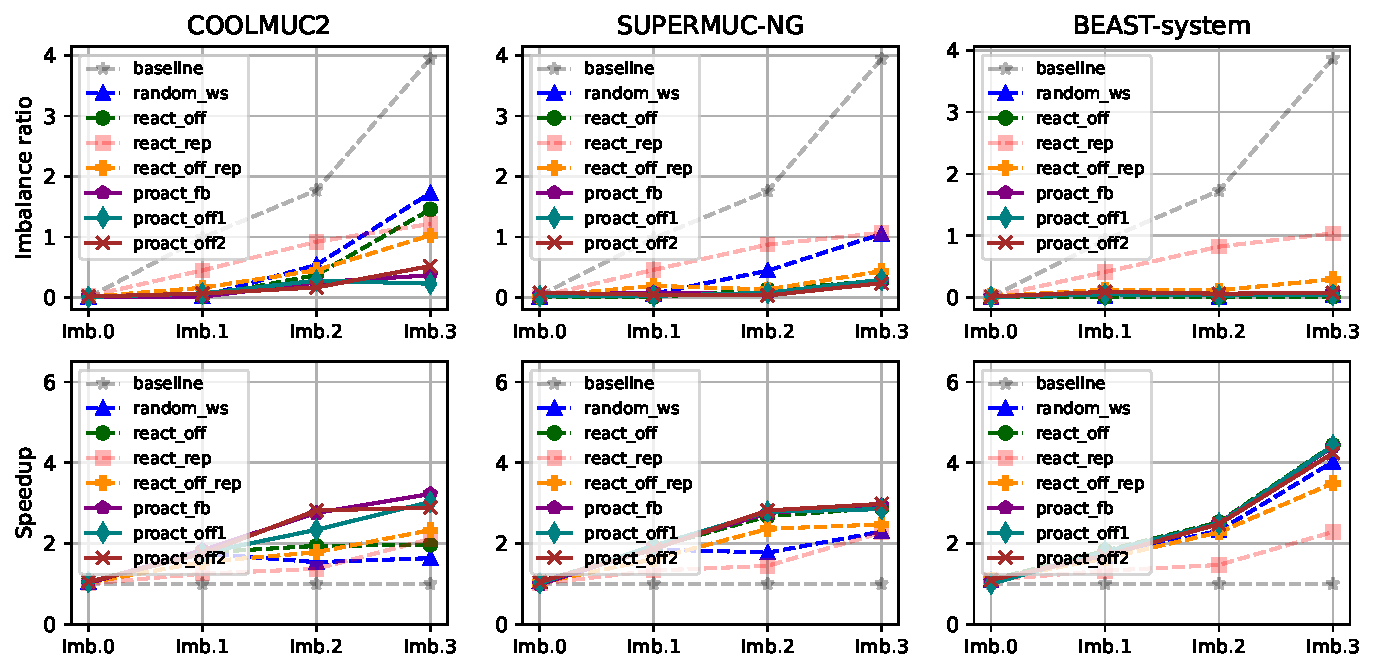
\includegraphics[scale=0.675]{./pictures/evaluation/eval_artificial_benchmark_mxm.pdf}
	\caption{A comparison of different load balancing methods on \texttt{MxM} through imbalance ratio and speedup.}
	\label{fig:eval_mxm_benchmarks}
\end{figure}

%\noindent \textbf{A. Experiments with synthetic micro-benchmark, \texttt{MxM}} \\
\subsection{Experiments with \texttt{MxM} matrix multiplication}
\label{subsec:exp_eval_lb_mxm}

The synthetic \texttt{MxM} is reproducible, where a task is defined by an \texttt{MxM} compute kernel. Given the tasks are independent and have uniform load if the matrix sizes are configured the same. We create different imbalance scenarios by varying the number of \texttt{MxM} compute tasks per MPI process as a given distribution. There are $4$ cases generated from no imbalance to high imbalance ratios (\texttt{Imb.0} - \texttt{Imb.3}). Due to permission on the systems CoolMUC2 and SuperMUC-NG at LRZ, we cannot adjust the core frequency to emulate performance slowdown, and the frequency is configured at a fixed level. Thereby, matrix sizes are the input parameters that mainly affect the accuracy of online load prediction on these two systems. Core frequency values fluctuate in the BEAST system, so the load prediction model still works with the input features of both application and system. For each run, \texttt{MxM} is set up $5$ iterations as $5$ execution phases of computing tasks, where the first iteration is used for load prediction, and the remaining iterations are used to evaluate load balancing methods.\\

The experimental results are presented in Figure \ref{fig:eval_mxm_benchmarks}. There are two rows of results corresponding to the sub-figures (sub-images), where the first row denotes imbalance ratios, the second row denotes speedup. From left to right, each sub-figure shows the corresponding results of each system, including CoolMUC2, SuperMUC-NG, and BEAST. Regarding the coordinates, the x-axis indicates imbalance scenarios in response to \texttt{Imb.0}, \texttt{Imb.1}, \texttt{Imb.2}, \texttt{Imb.3}, while the y-axis indicates the evaluation values, imbalance ratio or speedup.\\

For evaluating imbalance ratios, we can see that the reactive load balancing methods \texttt{react\_off} and \texttt{react\_off\_rep} are competitive. However, these methods show that the imbalance can still be improved with a high imbalance scenario such as \texttt{Imb.3}. For example, the values of $R_{imb}$ in this case are still high on CoolMUC2, $\approx$ 1.7 with \texttt{random\_ws}, 1.5 - 1.1 with \texttt{react\_off} and \texttt{react\_off\_rep}. With our approach, the proactive load balancing methods \texttt{proact\_fb}, \texttt{proact\_off1}, and \texttt{proact\_off2} reduce the case \texttt{Imb.3} under $0.6$. On SuperMUC-NG and the BEAST system, the overhead of load balancing and task migration is mitigated by better computation speed and interconnection network compared to CoolMUC2. This is beneficial for a compute-bound microbenchmark like \texttt{MxM}. Especially, the results in BEAST show that the reactive load balancing methods are still robust.\\

Corresponding to the imbalance ratio results, we show the speedup results on the second row of Figure \ref{fig:eval_mxm_benchmarks}. The three proactive load balancing methods gain an improvement in CoolMUC2 $1.2\times$ speedup compared to \texttt{react\_off} and $1.4\times$ to \texttt{random\_ws} in average;  $1.64\times$ speedup compared to \texttt{react\_off} and $1.97\times$ to \texttt{random\_ws} in maximum. In SuperMUC-NG, we do not gain much improvement in average, where the methods \texttt{proact\_fb}, \texttt{proact\_off1}, and \texttt{proact\_off2} only get $1.2\times$ compared to \texttt{random\_ws}, and approximate the speedup of reactive methods. Similarly, in the BEAST system, the performance of proactive methods also approximates the reactive methods. Reactive load balancing still shows resistance for different imbalance scenarios on BEAST.\\

%\begin{minipage}[t]{0.5\textwidth}
%%\centering
%%\caption{Case 2: Imbalance Ratio (\texttt{imb.2}}
%\captionof{table}{Case 2: Imbalance Ratio (\texttt{imb.2})}
%\label{tab:imb2_overhead_info}
%\scalebox{0.5}{
%\begin{tabular}{|l|l|l|l|}
%\hline
%\multicolumn{1}{|c|}{\textbf{AVERAGE}}   & \textbf{COOLMUC2} & \textbf{SUPERMUC-NG} & \textbf{BEAST-system} \\ \hline
%\textbf{$\sum$(\#migrated tasks) over ranks}      & 965.20    &  1017.60   & 1179.60     \\ \hline
%%\textbf{migration throughput (\texttt{tasks/s})}  & 182.580   &  243.150   & 233.637    \\ \hline
%\textbf{\#balancing calculation calls}            & 47965.85  &  10755.78  & 202010.57   \\ \hline
%\textbf{cost/balancing calculation ($\mu$s)}      & 0.313387  &  0.314263  & 0.126097    \\ \hline
%\end{tabular}}
%\end{minipage}
%\begin{minipage}[t]{0.5\textwidth}
%%\centering
%\captionof{table}{Case 3: Imbalance Ratio (\texttt{imb.3})}
%\label{tab:imb3_overhead_info}
%\scalebox{0.5}{
%\begin{tabular}{|l|l|l|l|}
%\hline
%\multicolumn{1}{|c|}{\textbf{AVERAGE}}   & \textbf{COOLMUC2} & \textbf{SUPERMUC-NG} & \textbf{BEAST-system} \\ \hline
%\textbf{$\sum$(\#migrated tasks) over ranks}      & 592.00   & 566.80    & 709.40     \\ \hline
%%\textbf{migration throughput (\texttt{tasks/s})}  & 140.396  & 200.841   & 170.027    \\ \hline
%\textbf{\#balancing calculation calls}            & 10534.00 & 3201.38   & 37528.60   \\ \hline
%\textbf{cost/balancing calculation ($\mu$s)}      & 0.403371 & 0.309864  & 0.129224   \\ \hline
%\end{tabular}}
%\end{minipage}

\begin{table}[t]
\centering
\caption{Scenario 2: Imbalance Ratio (\texttt{imb.2})}
\label{tab:imb2_overhead_info}
\scalebox{0.775}{
\begin{tabular}{|l|l|l|l|}
\hline
\multicolumn{1}{|c|}{\textbf{AVERAGE}}   & \textbf{COOLMUC2} & \textbf{SUPERMUC-NG} & \textbf{BEAST-system} \\ \hline
\textbf{$\sum$(\#migrated tasks) over ranks}      & 965.20    &  1017.60   & 1179.60     \\ \hline
%\textbf{migration throughput (\texttt{tasks/s})}  & 182.580   &  243.150   & 233.637    \\ \hline
\textbf{\#balancing calculation calls}            & 47965.85  &  10755.78  & 202010.57   \\ \hline
\textbf{cost/balancing calculation ($\mu$s)}      & 0.313387  &  0.314263  & 0.126097    \\ \hline
\end{tabular}}
\end{table}

\begin{table}[t]
\centering
\caption{Scenario 3: Imbalance Ratio (\texttt{imb.3})}
\label{tab:imb3_overhead_info}
\scalebox{0.775}{
\begin{tabular}{|l|l|l|l|}
\hline
\multicolumn{1}{|c|}{\textbf{AVERAGE}}   & \textbf{COOLMUC2} & \textbf{SUPERMUC-NG} & \textbf{BEAST-system} \\ \hline
\textbf{$\sum$(\#migrated tasks) over processes}      & 592.00   & 566.80    & 709.40     \\ \hline
%\textbf{migration throughput (\texttt{tasks/s})}  & 140.396  & 200.841   & 170.027    \\ \hline
\textbf{\#balancing calculation calls}            & 10534.00 & 3201.38   & 37528.60   \\ \hline
\textbf{cost/balancing calculation ($\mu$s)}      & 0.403371 & 0.309864  & 0.129224   \\ \hline
\end{tabular}}
\end{table}

To explain how the reactive methods are still robust on BEAST, we present the profiled data of balancing operations. This is the detailed information of \texttt{react\_off} (which denotes reactive task offloading and the best reactive method in the experiments above) in the cases \texttt{imb.2} and \texttt{imb.3}, shown in Table \ref{tab:imb2_overhead_info} and Table \ref{tab:imb3_overhead_info} respectively. Each table has four columns, where the first column highlights three profiled information as explained below. The remaining columns are the profiled information that \texttt{react\_off} is run on the corresponding systems, CoolMUC2, SuperMUC-NG, and BEAST.
\begin{itemize}
	\item $\sum$(\#migrated tasks) over processes: the average sum of how many tasks are migrated. This value gives an overview of the number of tasks moved around processes.
	\item \#balancing calculation calls: the average number of reactive balancing calculation calls. This value denotes the operations for checking queue status and calculating imbalance conditions performed by $Tcomm$.
	\item cost/balancing calculation ($\mu$s): the average cost per balancing calculation call in microseconds ($\mu$s). This value denotes the overhead of running the operation that calculates imbalance ratios and detect an imbalance.
\end{itemize}

These three values are first calculated by average over the number of iterations, then second by average over the number of processes. A large or small number of $\sum$(\#migrated tasks) over processes does not mainly indicate good or bad migration because there could be some wrong task migration at an incorrect reactive decision. However, this value can show the availability and capability of each system in migrating tasks. With \#balancing calculation calls, a larger number shows $Tcomm$ works more active in checking imbalance status. \\

As the results in both Table \ref{tab:imb2_overhead_info} and Table \ref{tab:imb3_overhead_info}, we can see that the balancing cost on BEAST is $\approx 2\times$ - $3\times$ lower than on SuperMUC-NG and CoolMUC2. The number of migrated tasks is also higher. The BEAST system has benefited from the migration throughput as well as the lower cost of balancing operations. $Tcomm$ is more reactive; therefore, even in the case of wrong task migration, it can migrate tasks back around. Furthermore, the interconnection network on BEAST is more stable because this system is used as a testbed. On SuperMUC-NG and CoolMUC2, a job running can be affected by other jobs using the same interconnection in the same rack.

%\noindent \textbf{B. Experiments with realistic application, Sam(oa)$^2$} \\
\subsection{Experiments with Sam(oa)$^2$}
\label{subsec:exp_eval_lb_samoa}

\begin{figure}[t]
  \centering
  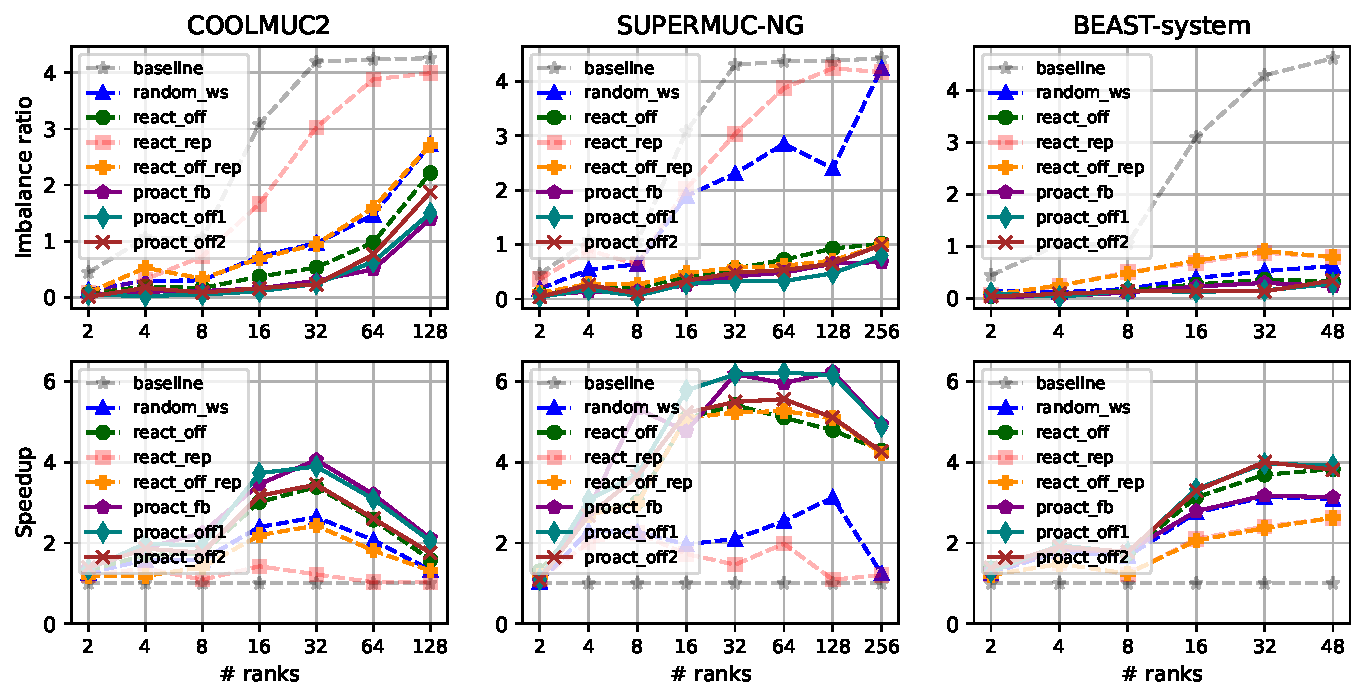
\includegraphics[scale=0.675]{./pictures/evaluation/eval_realistic_usecase_samoa_osc.pdf}
	\caption{Comparison of different load balancing methods on Sam(oa)$^2$ simulating the scenario of oscillating lake.}
	\label{fig:eval_samoa_osc}
\end{figure}

Sam(oa)$^2$ is set up by running a 100 time-steps simulation. The simulation scenario is again oscillating lake, where tasks are defined by traversing sections (like cells in the grid) that we have explained in Chapter \ref{ch:PADLB}, Section \ref{sec:PADLB-MLbasedTaskOffload} on Page \pageref{subsubsec:samoa-online-prediction}. The load of tasks in a process can be changed dynamically due to the adaptive mesh refinement algorithm \cite{rannabauer2018samoaaderdg}, which is related to wetting, drying, and the limiter applied to several mesh cells. We use standard configurations, where tasks are fine-grained, and the number of tasks per process depends on simulation scenario scale, i.e., the number of sections per mesh region. \\

In Sam(oa)$^2$, there are several parameters\footnote{https://github.com/meistero/Samoa} to set up a simulation scenario, e.g., the number of sections (\texttt{sections}), number of threads (\texttt{threads}), number of nodes (\texttt{nodes}), number of iterations (\texttt{nmax}), boundary size (\texttt{boundary\_size}), etc. On the side of a task-based programming framework, application is considered as a black box. Hence, we are simly concerned with the parameters in Sam(oa)$^2$ that define tasks and affect imbalance with the scale of execution. Such the default configuration, we set up \texttt{sections} $=16$, \texttt{threads} $=13$, \texttt{nodes} $=32$, \texttt{nmax} $=50$. In detail,
\begin{itemize}
	\item \texttt{sections}: the number of sections created and executed within a thread.
	\item \texttt{threads}: the number of threads spawn in a process. Multiplying \texttt{threads} with \texttt{sections} determines the number of tasks defined and assigned to a process. For example, here we have $13$ $\times$ $16$ = $208$ tasks per process.
	\item \texttt{nodes}: the number of compute nodes that are required and allocated on HPC clusters. If we multiply the number of tasks per process with \texttt{nodes}, the total number of tasks is $208$ $\times$ $32$ $=$ $6656$ tasks in total.
	\item \texttt{nmax}: the number of time steps that run the simulation. Depending on a simulated scenario and algorithm used in Sam(oa)$^2$, this value can regulate the number of actual iterations run in practice, e.g., $2$ $\times$ \texttt{nmax} is the number of actual iterations. Therefore, this case has $100$ iterations.
\end{itemize}

By characterizing the behavior of Sam(oa)$^2$, we observe that the load of tasks is uniform, and task distribution is fine-grained. Nonetheless, the load values can be susceptible to numerical algorithms. The load value per task is not large but prone to fluctuations. Therefore, many tasks per node can be affected by fluctuations in system performance slowdown, leading to an imbalance.\\

For the evaluation, we vary the number of processes on each system with two MPI processes per node, and each process uses full cores of a CPU socket. The experiments can show scalability and adaptation in various methods, especially with different interconnection networks on three systems. Similar to the format of Figure \ref{fig:eval_mxm_benchmarks} in the previous subsection, the experimental results are shown in Figure \ref{fig:eval_samoa_osc}. There are also two rows showing the results. The first row points to imbalance ratio, while the second row points to speedup. Each sub-figure has the x-axis showing the scale of processes used to run the experiment, while the y-axis shows the imbalance and speedup values.\\

Overall, the reactive and proactive load balancing methods perform better than work stealing. With reactive load balancing, \texttt{react\_off} is shown as the best method in most of the cases, while (\texttt{react\_rep}) is worse because of the cost of speculative task replication. Nevertheless, their combination \texttt{react\_off\_rep} could help the cases from $16$ processes (MPI ranks) on CoolMUC2 and BEAST. Based on profiling the execution behavior of \texttt{react\_rep}, we notice that the speculative task replication strategy has difficulty dealing with the imbalance of consecutive underloaded processes. For instance, without prior knowledge, we have to fix a certain number of replicated tasks and the process victim for replication.\\

With our proactive approach, we use online prediction to provide load information guiding task offloading. The methods \texttt{proact\_fb}, \texttt{proact\_off1}, and \texttt{proact\_off2} show an improvement in the high imbalance cases ($\geq 8$ processes), where \texttt{proact\_fb} and \texttt{proact\_off1} are competitive. The benefit that makes our methods better is predicted load information at runtime. This helps reduce the number of wrong task migration decisions. Simultaneously, we can better estimate the appropriate number of tasks and potential processes for migration.\\

Especially on CoolMUC2 and SuperMUC-NG, \texttt{proact\_fb} and \texttt{proact\_off1} achieve the best performance. Differing from the results of \texttt{MxM}, we gain the best performance with \texttt{proact\_fb} and \texttt{proact\_off1} on SuperMUC-NG. In particular, the performance gain is $1.2\times$ speedup compared to \texttt{react\_off} and $2.3\times$ to \texttt{random\_ws} in average; $1.7\times$ speedup compared to \texttt{react\_off} and $3.9\times$ to \texttt{random\_ws} in maximum. On CoolMUC2, Sam(oa)$^2$ with our methods gains around $1.2\times$ speedup compared to \texttt{react\_off} and $1.4\times$ to \texttt{random\_ws} in average; $1.3\times$ speedup compared to \texttt{react\_off} and $1.6\times$ to \texttt{random\_ws} in maximum. Similar to the results of \texttt{MxM}, the performance improvement of proactive load balancing on BEAST is insignificant and approximates the reactive methods.\\

With two proactive task offloading methods, \texttt{proact\_off2} has some delay for encoding a set of tasks when the data is large. Therefore, if an overloaded rank has multiple victims, the second victim must wait longer to proceed the first one.\\

In principle, proactive task offloading must depend on the accuracy of load prediction models. However, the features characterized by an online scheme at runtime can reflect the execution behavior adaptively. Besides, our expected accuracy of prediction models does not need to be too high, which means an acceptable result to estimate the load difference among processes is enough for load balancing. Therefore, the proactive load balancing scheme is feasible to perform proactive task offloading. 

% To be extended, we can combine reactive and proactive approaches to improve each other.

% In maximum, we gain  $\approx 1.1\times$ to \texttt{react\_off}. The reactive approaches on SuperMUC-NG and BEAST still work well in this case.\\
% They have applied the same proactive scheme for predicting load and balancing algorithms but different migration strategies. All compared methods are addressed in Table \ref{tab:compare_methods}.
% It indicates that the $W_{par}$ and waiting-time values between ranks are low.

\section{Evaluation of Co-scheduling Tasks across Multiple Applications} \label{sec:evalulate_coschedule_tasks}

As addressed in Chapter \ref{ch:PADLB}, Section \ref{sec:PADLB-CoschedulingTask}, the experiments of co-scheduling tasks across multiple applications have to be emulated on HPC systems. We define different tasks of different applications in the same executable to emulate multiple runs simultaneously. There are three experiments to show the applicability and performance of our co-scheduling extension.
\begin{itemize}
	\item Experiment 1: aims to show the feasibility of co-scheduling tasks across two applications. We use two types of \texttt{MxM} compute tasks accounting for two \texttt{MxM} applications. The results are shown in Table \ref{tab:coschedule_two_apps}.
	\item Experiment 2: aims to vary the proportion of idle slots between two applications. This experiment can show the advantage when tasks from one application can be co-scheduled to another, corresponding to the idle proportion. We also use two types of \texttt{MxM} compute tasks accounting for two different \texttt{MxM} applications. The results are shown in Figure \ref{fig:eval_coschedule_varied_idles}.
	\item Experiment 3: aims to show the benefit of co-scheduling tasks across different microbenchmarks, including \texttt{MxM}, Cholesky, Jacobi, and Nbody. The results of this experiment are shown in Figure \ref{fig:eval_coschedule_multi_apps}
\end{itemize}

\begin{table}[t]
\caption{An experiment of co-scheduling tasks across two applications under randomized task generation and imbalance ratios.}
\label{tab:coschedule_two_apps}
\scalebox{0.925}{
\begin{tabular}{|l|ll|l|l|l|l|l|}
\hline
\multirow{2}{*}{\textbf{Imb.Case}} & \multicolumn{2}{c|}{\textbf{\#tasks}} & \multirow{2}{*}{\textbf{\#shared tasks}} & \multirow{2}{*}{\textbf{$C_{max}$}} & \multirow{2}{*}{\textbf{$C^{'}_{max}$}} & \multirow{2}{*}{\textbf{Overhead}} & \multirow{2}{*}{\textbf{Speedup}} \\ \cline{2-3}
     & \multicolumn{1}{l|}{\textbf{App.1}} & \textbf{App.2} &  &  &  &  &   \\ \hline
 C1-$R_{imb} = 0.06$ & \multicolumn{1}{l|}{ 58}  &   51  &   3  & 21.935 & 17.253 &  8.46\%  & 1.27$\times$ \\ \hline
 C2-$R_{imb} = 0.38$ & \multicolumn{1}{l|}{100}  &   45  &  27  & 37.799 & 22.924 &  8.27\%  & 1.65$\times$ \\ \hline
 C3-$R_{imb} = 0.04$ & \multicolumn{1}{l|}{105}  &  113  &   4  & 42.982 & 34.286 &  7.99\%  & 1.25$\times$ \\ \hline
 C4-$R_{imb} = 0.29$ & \multicolumn{1}{l|}{121}  &   66  &  27  & 46.601 & 29.483 &  8.43\%  & 1.58$\times$ \\ \hline
 C5-$R_{imb} = 0.51$ & \multicolumn{1}{l|}{140}  &   46  &  47  & 52.522 & 29.259 &  8.38\%  & 1.79$\times$ \\ \hline
 C6-$R_{imb} = 0.27$ & \multicolumn{1}{l|}{154}  &   89  &  32  & 57.976 & 38.180 &  8.38\%  & 1.52$\times$ \\ \hline
 C7-$R_{imb} = 0.31$ & \multicolumn{1}{l|}{190}  &  101  &  44  & 72.711 & 43.701 &  9.36\%  & 1.66$\times$ \\ \hline
\end{tabular}}
\end{table}

In Experiment 1, a given imbalance scenario is set up before two applications run, where one is intended to configure fewer compute tasks but more idle slots, while one has more compute tasks. The number and data size of tasks are randomized to generate non-uniform load and random imbalance levels. Table \ref{tab:coschedule_two_apps} details the experiment results with eight columns. The first column indicates the label of imbalance cases, marked from C1 to C7 and associated with the values of $R_{imb}$. The second and third columns show the number of tasks that are randomly created on each application, ``$App.1$'' and ``$App.2$''. For example, in case C1, $App.1$ has $58$ tasks, while $App.2$ has $51$ tasks, $R_{imb}$ is $0.06$. The column ``\#shared tasks'' indicates the number of tasks that are co-scheduled across $App.1$ and $App.2$ to make them both improve the performance. Following that, the remaining columns show the evaluation metrics in:
\begin{itemize}
	\item $C_{max}$: the completion time without co-scheduling tasks. This value is measured by the maximum completion time between $App.1$ and $App.2$.
	\item $C^{'}_{max}$: the completion time with co-scheduling tasks. Similarly, this value is also measured by the maximum completion time between $App.1$ and $App.2$.
	\item Overhead: the consumped time is measured when the co-scheduler is triggered and spent time to take action on task migration.
	\item Speedup: the ratio between $C_{max}$ and $C^{'}_{max}$.
\end{itemize}

By applying co-scheduling tasks, the overloaded application sends an estimated number of tasks to another application. Note that task input arguments are sent from the side of the original processes in $App.1$, while only task results are sent back when the execution is done on the remote side, $App.2$. As a result, Table \ref{tab:coschedule_two_apps} shows an improvement with the values $C^{'}_{max}$ compared to $C_{max}$. Between $App.1$ and $App.2$, the application with idle slots can be filled up by compute tasks received from the other application.\\

Regarding the overhead, our approach shows that the cost is under $10\%$ in this case, compared to the completion time of applications. With the isolated $Tcomm$, co-scheduling tasks across two applications is feasible. $Tcomm$ is asynchronously managed; therefore, we can overlap communication with computation, and the overhead has a small impact on other threads. The speedup columns show positive results, particularly in the high imbalance cases such as C4, C5, C7. Generally, these test cases are considered as reproducible test cases for co-scheduling tasks between two applications. When one is busier with more compute tasks, the other can share available tasks.\\


\begin{figure}[t]
  \centering
  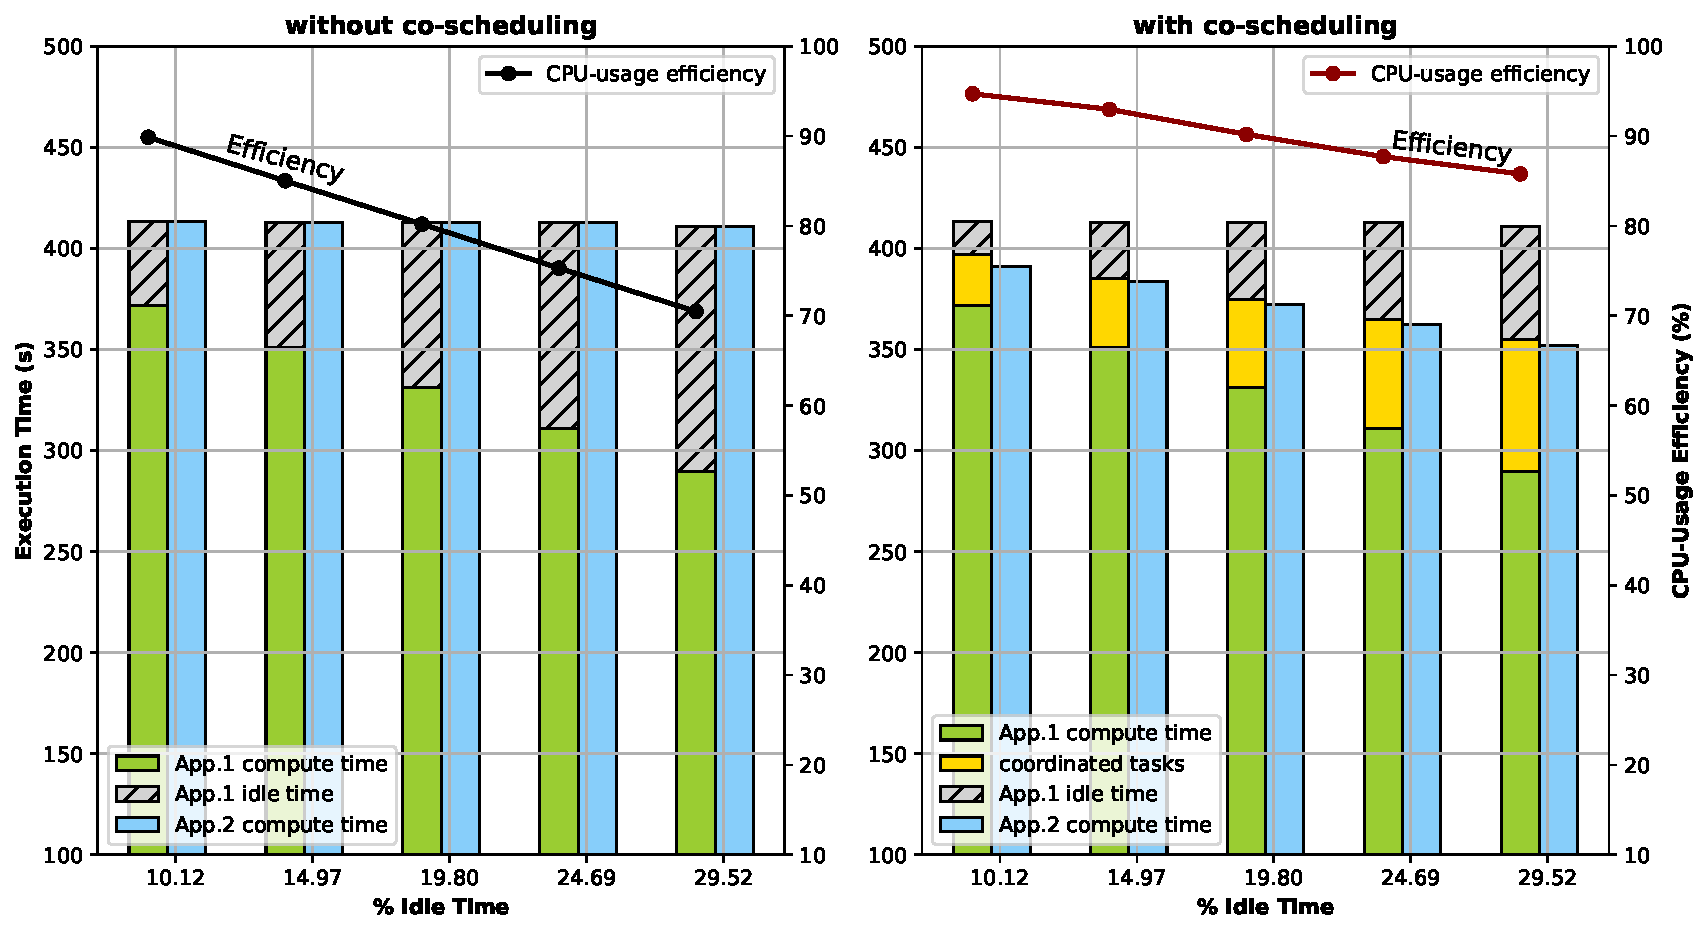
\includegraphics[scale=0.45]{./pictures/evaluation/eval_coschedule_2apps_varied_idles.pdf}
	\caption{An experiment of co-scheduling tasks across two applications under varied idle slots.}
	\label{fig:eval_coschedule_varied_idles}
\end{figure}

\begin{figure}[t]
  \centering
  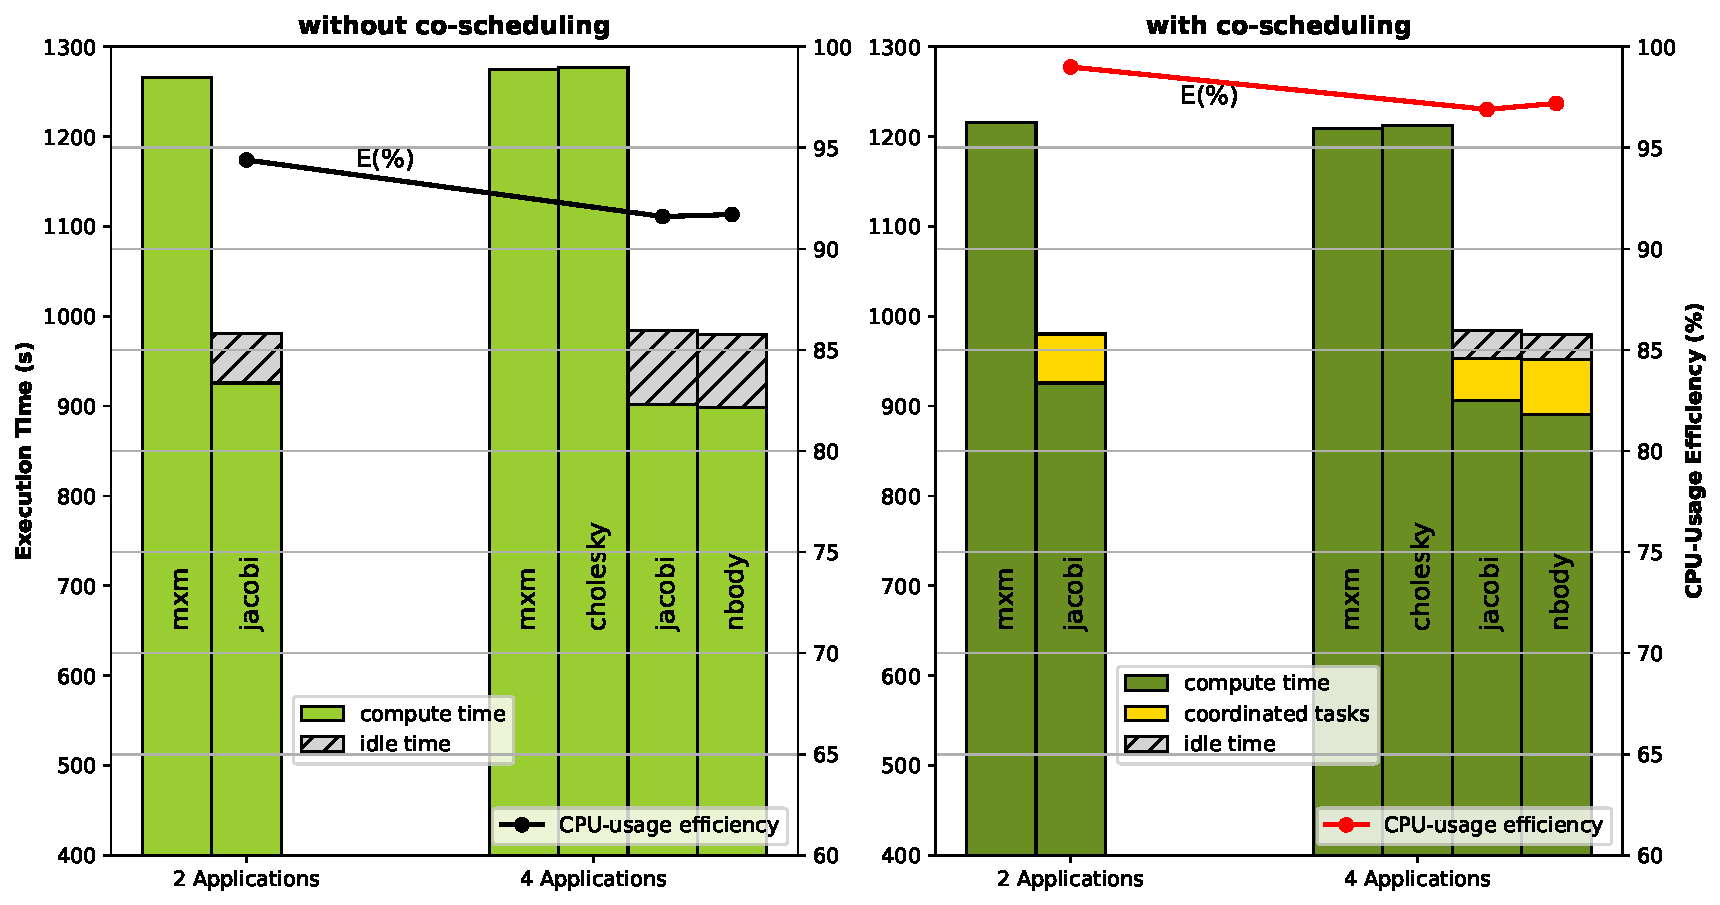
\includegraphics[scale=0.425]{./pictures/evaluation/eval_coschedule_multi_apps.pdf}
	\caption{An experiment of co-scheduling tasks across different applications.}
	\label{fig:eval_coschedule_multi_apps}
\end{figure}

In Experiment 2, we still use two types of \texttt{MxM} compute tasks accounting for two \texttt{MxM} applications running simultaneously. One application has I/O tasks representing idle slots, where we can vary the length of idle slots. This experiment evaluates how many tasks can be migrated to fill the idle slots for co-scheduling. Furthermore, it shows how much improvement we can obtain. The results are shown in Figure \ref{fig:eval_coschedule_varied_idles} with two figures: one on the left indicates the experiments without co-scheduling, and one on the right indicates the experiments with co-scheduling. In each figure, the x-axis shows the proportion of idle slots over the completion time, from $\approx 10\%$ to $\approx 30\%$. The y-axis is a double axis, where the left one denotes application execution time or completion time, the right one denotes CPU usage efficiency (in percentage $\%$). The CPU usage efficiency is calculated by $E = \frac{\sum CPU_{\texttt{compute\_time}}}{C_{max} \times \texttt{num\_cores}}$, where the sum means all computation time measured by all CPU cores, $C_{max}$ is the completion time in parallel, and $\texttt{num\_cores}$ is the number of used CPU cores.\\

Principally, the ideal CPU utilization efficiency is $100\%$, but we cannot reach this maximum due to idle slots. Therefore, co-scheduling tasks can reduce idle slots in $App.1$ and increase the CPU usage efficiency in $App.2$. In Figure \ref{fig:eval_coschedule_varied_idles} (left), the area of idle in $App.1$ is marked with the color in grey. In Figure \ref{fig:eval_coschedule_varied_idles} (right), we can see that this area of $App.1$ is filled with the execution time of migrated tasks from App.2 (denoted by \texttt{coordinated tasks}). Corresponding to the length of idle slots, the number of offloaded tasks is estimated by the proposed algorithm in Chapter \ref{ch:PADLB}, Section \ref{sec:PADLB-CoschedulingTask}. \\

In Experiment 3, we perform co-scheduling on different micro-benchmarks representing tasks from different applications. The results are shown in Figure \ref{fig:eval_coschedule_multi_apps} also with two figures, where one on the left side indicates the experiments without co-scheduling, while one on the right side indicates the experiments with co-scheduling. Each figure highlights two cases, a case with two applications (\texttt{MxM} and Jacobi) and a case with four applications running simultaneously (\texttt{MxM}, Jacobi, Cholesky, and Nbody). The x-axis of each figure denotes the case labels associated with the number of involved applications. Similar to Figure \ref{fig:eval_coschedule_varied_idles}, the y-axis (left) denotes completion time in seconds ($C_{max}$), while the y-axis (right) denotes CPU usage efficiency in $\%$. The length of stacked bars in Figure \ref{fig:eval_coschedule_multi_apps} shows the length of $C_{max}$, where the grey area with stripes indicates the accumulated time of idle slots. The yellow area indicates execution time occupied by another application's remote tasks (migrated tasks). The value of line charts indicates CPU usage efficiency (higher is the better), following the y-axis on the right side. \\

Note that the results in both figures are the average results collected by at least $5$ times runs per experiment. Thereby, the height of stacked bars corresponding to the cases of without and with co-scheduling cannot be $100\%$ equal due to noise at system and runtime. As a result, the applications with more compute tasks can share computation slots with the others, e.g., tasks in \texttt{MxM} and Cholesky are shared to coordinate with tasks in Jacobi and Nbody. The idle slots are replaced with remote task execution. After execution, the results of remote tasks are sent back to the processes of the original applications. The line chart in this experiment shows an average of $5\%$ in CPU usage efficiency compared to the cases without co-scheduling tasks.\\

Our co-scheduling method can work with task-based parallel applications when we know a given distribution of tasks before execution. In the case, if tasks are generated dynamically and unpredictably, this co-scheduling method might have some risks. Due to abnormal behaviors, automatic task generation makes it difficult to manage the movement of tasks among different applications. Nevertheless, our work shows that emerging task-based parallel models can facilitate parallel execution via task abstraction. With the co-scheduling scheme, we can support portability in
\begin{itemize}
	\item Predicting idle slots as well as task execution time.
	\item Offloading tasks proactively from a busy process to an idle one, following a co-scheduling algorithm.
	\item Getting benefits in hiding idle and increasing computing resource usage by exploiting the repeated behaviors of scientific simulations in HPC.
\end{itemize}

% In detail, only the task's arguments are sent forward to the idle side, and the busy side gets back their results after the execution of remote tasks is done.\\

%\vfill
%\section*{Chapter Summary}
%\label{sec:Eval-Summary}
%
%Chapter~\ref{ch:Evaluation} provides a brief evaluation and self assessment of
%the work at hand.
%This is achieved by providing a summary for the assessment of the requirements
%for an \pne management system of Chapter~\ref{ch:Motivation} for the developed \gls*{OIEPrefmodel}
%(presented in full in  App.~\ref{sec:Eval-Requirements}).
%
%This is followed by a discussion on the limited fulfillment of a selection of
%requirements, presented in Section~\ref{sec:Eval-Comparison}.
%The chapter is complemented with a short discussion on use-cases in
%Section~\ref{sec:Eval-Discussion}.
%The chapter (supplemented by App.~\ref{App:Ass}) forms the first part of the
%last step of the thesis method the \textit{evaluation and evolution}, which is
%continued in the future work discussion of Chapter~\ref{ch:Future}.
%\begin{figure}[H]
%    \centering
%    \resizebox{.98\textwidth}{!}{%
%        %%define
\def\radius{6cm}

\begin{tikzpicture}

\node[draw=white]()at(-9.2,-5.0){};
\node[draw=white]()at(-9.2,+5.0){};
\node[draw=white]()at(+9.2,-5.0){};
\node[draw=white]()at(+9.2,+5.0){};

%LEFT
\draw[draw=black,fill=white,line width=4.2pt,->,>=stealth] ([shift=(220:3.2cm)]-2.9,0) arc (218: 95:3.2cm);
\draw[draw=black,line width=4.2pt,->,>=stealth] ([shift=( 90:3.2cm)]-2.9,0) arc ( 90:  0:3.2cm);
\draw[draw=lightgray,line width=4.2pt,->,>=stealth] ([shift=(355:3.2cm)]-2.9,0) arc (355:232:3.2cm);
\draw[loosely dotted,draw=black,line width=4.2pt,-,>=stealth] ([shift=(355:3.2cm)]-2.9,0) arc (355:293.5:3.2cm);


%Eintritt
\draw[line width=4.2pt,<-,>=stealth] ([shift=( 225:3.2cm)]-2.9,0)++(-0.15cm,-0.1cm)
arc (385:375:2cm)
arc (385:270:0.5cm);

%LABELs
\node[left,align=right](PDRM-label)at(-5.4,-3.0){Problem definition};
\node[left=0.1cm of PDRM-label,circle, black, draw](a) {1};
\node[text=black,right,align=left](PARM-label)at(-5.875,-0.0){Problem domain\\analysis};
\node[draw=black,left=0.40cm of PARM-label,circle, black, draw](b) {2};
\node[text=black,left,align=right](KRM-label) at(-0.8,+2.0){Reference model\\construction};
\node[draw=black,left=0.1cm of KRM-label,circle, black, draw](c) {3};
\node[text=black,left,align=left](ERM-label) at(-0.65,-2.20){Evaluation and\\evolution};
\node[draw=black,left=0.1cm of ERM-label,circle, black, draw](d) {4};

\draw[draw=black,decoration={brace,mirror,raise=5pt,amplitude=14pt},decorate]
  (-6.0,-3.8) -- node[below=20pt] {Reference model building} (-0.2,-3.8);


%RIGHT
\draw[draw=black,line width=4.2pt,->,>=stealth] ([shift=( 95:3.2cm)]+2.9,0) arc ( 95:180:3.2cm);
\draw[draw=black,line width=4.2pt,->,>=stealth] ([shift=(185:3.2cm)]+2.9,0) arc (185:310:3.2cm);
\draw[draw=black,line width=4.2pt,->,>=stealth] ([shift=(-45:3.2cm)]+2.9,0) arc (-45: 70:3.2cm);

%Eintritt
\draw[draw=black,line width=4.2pt,<-,>=stealth] ([shift=( 93:3.2cm)]+2.9,0)++(0,0.1cm) arc (270:340: 1.2cm);
%Austritt
\draw[draw=black,line width=4.2pt,->,>=stealth] ([shift=( 72:3.2cm)]+2.9,0)++(0,0.1cm) arc (200:100:0.5cm) arc (100:90:3.2cm);
%Fill the white spot in the out arrow!
\filldraw[black] (4.55,3.840) circle (2pt) node[]{};

%LABELs
\node[text=black,left,align=left](SPD-label)at(+3.4,+4.0){HPC system specific\\problem description};
\node[draw=black,left=0.1cm of SPD-label,circle, black, draw](a) {a};
%\node[text=black,right,align=left](SR-label)at(+0.8,+2.0){Requirements\\identification};
%\node[draw=black,right=0.1cm of SR-label,circle, black, draw](b) {b};
\node[text=black,right,align=left](SR-label)at(+1.6,+2.0){Identification of\\requirements};
\node[draw=black,left=0.1cm of SR-label,circle, black, draw](b) {b};
\node[text=black,right,align=right](SMS-label)at(+0.575,-2.15){Reference model- \\/ Architecture-\\ selection};
\node[draw=black,right=0.1cm of SMS-label,circle, black, draw](c) {c};
\node[text=black,left,align=right](SMC-label)at(+5.9,-0.0){Architecture\\construction\\/ -adaptation};
\node[draw=black,right=0.40cm of SMC-label,circle, black, draw](d) {d};
\node[text=black,right,align=left](SSM-label)at(+4.9,+3.825){Specific architecture};
\node[draw=black,right=0.1cm of SSM-label,circle, black, draw](e) {e};

\draw[text=black,draw=black,decoration={brace,mirror,raise=5pt,amplitude=14pt},decorate]
  (0.2,-3.8) -- node[below=20pt] {Application of the reference model} (6.0,-3.8);


\end{tikzpicture}

%    }
%    \caption[Method Completion After Chapter 5.]{%
%        Method completion after Chapter 5.}
%    \label{fig:Method-Completion5}
%\end{figure}
